\documentclass[conference]{IEEEtran}
% \IEEEoverridecommandlockouts
% The preceding line is only needed to identify funding in the first footnote. If that is unneeded, please comment it out.
\usepackage{cite}
\usepackage{amsmath,amssymb,amsfonts}
\usepackage{algorithm}
\usepackage{algorithmicx}
\usepackage[noend]{algpseudocode}
\usepackage{graphicx}
\usepackage{textcomp}
\usepackage{xcolor}
\usepackage{tikz}
\usepackage{pgfplots}
\usepackage{hyperref}

\def\BibTeX{{\rm B\kern-.05em{\sc i\kern-.025em b}\kern-.08em
    T\kern-.1667em\lower.7ex\hbox{E}\kern-.125emX}}
\begin{document}

\title{Towards Triangle Counting on GPU using Stable Radix binning\\
}

\author{\IEEEauthorblockN{Nishith Tirpankar}
\IEEEauthorblockA{\textit{School of Computing} \\
\textit{University of Utah}\\
Salt Lake City, USA \\
tirpankar.n@utah.edu}
\and
\IEEEauthorblockN{Hari Sundar}
\IEEEauthorblockA{\textit{School of Computing} \\
\textit{University of Utah}\\
Salt Lake City, USA \\
hari@cs.utah.edu}
% \and
% \IEEEauthorblockN{3\textsuperscript{rd} Given Name Surname}
% \IEEEauthorblockA{\textit{dept. name of organization (of Aff.)} \\
% \textit{name of organization (of Aff.)}\\
% City, Country \\
% email address}
% \and
% \IEEEauthorblockN{4\textsuperscript{th} Given Name Surname}
% \IEEEauthorblockA{\textit{dept. name of organization (of Aff.)} \\
% \textit{name of organization (of Aff.)}\\
% City, Country \\
% email address}
% \and
% \IEEEauthorblockN{5\textsuperscript{th} Given Name Surname}
% \IEEEauthorblockA{\textit{dept. name of organization (of Aff.)} \\
% \textit{name of organization (of Aff.)}\\
% City, Country \\
% email address}
% \and
% \IEEEauthorblockN{6\textsuperscript{th} Given Name Surname}
% \IEEEauthorblockA{\textit{dept. name of organization (of Aff.)} \\
% \textit{name of organization (of Aff.)}\\
% City, Country \\
% email address}
}

\maketitle

\begin{abstract}
This document is a model and instructions for \LaTeX.
This and the IEEEtran.cls file define the components of your paper [title, text, heads, etc.]. *CRITICAL: Do Not Use Symbols, Special Characters, Footnotes, 
or Math in Paper Title or Abstract.
\end{abstract}

\begin{IEEEkeywords}
component, formatting, style, styling, insert
\end{IEEEkeywords}

\section{Introduction}
\subsection{Graph algorithms overview}
A number of data and network analytics questions on relational data can be posed as graph problems. For example, the transitivity or clustering coefficient tells us how clustered the nodes in a graph are. Clustered or small world networks having large value of clustering co-efficient have enhanced signal-propagation speed, synchronizability and computational power\cite{b1}. Nodes in sub-graphs with this property can be targetted for quick or low energy information disbursement. Another example involves finding the count and presence of certain structures in a graph. Identifying clusters of these patterns\cite{b2} or sub-graphs can indicate classes of predators in a food-web or interactions between sensors and effectors in a neural network\cite{b3}. A commonly occuring use case is of recommendations to connect with friends of friends in large social networks. It can be computed using the length of the path between two users\cite{b4}.
\subsection{Triangle counting as an application}
A k-truss is a maximal subgraph of a given graph such that each edge in it is contained in at least k-2 triangles. The k-truss in a graph is a sub-graph all the applications mentioned here can use. Triangles are the simplest subgraph in a graph. Counting the number of triangles in a graph is building block that can be used in finding the k-truss\cite{b5}. This makes triangle counting such a lucritive problem for the sub-graph isomorphism challenge\cite{b6}.
\subsection{Different approaches - set intersection/Linear algebra/map reduce/approximation methods for triangle counting}
Among the prominent methods for computing the count of triangles are ones using set intersection, linear algebra, map reduce and approximation methods. Set intersection algorithms \cite{b7} involve computing a set of all the possible edges that could generate triangles and counting the number of intersections with the original adjacency list. Innovations in the ordering of the members of the sets as well as ease of distribution of the work among multiple processes makes this class of algorithms highly performant\cite{b8} and ideal for implementation on shared memory systems. This class of algorithms is what inspired our work. Linear algebra approaches involve variantions of $\sum_{i,j}A^2\circ A$ where $A$ is the adjacency matrix\cite{b6}. One variantion involves splitting up the adjacency matrix into lower and upper triangular matrices not including the diagonal $A = L + U$. The product $B = L*U$ counts the number of paths of length 2 in the graph. Finding if the wedges close by performing a Hadamard product $C= A\circ B$ gives us the triangle count $\sum_{ij}(C)/2$\cite{b10, b9}. Map reduce approaches use frameworks such as Hadoop and distribute the adjacency lists among nodes arbitrarily. For a more detailed overview refer to \cite{b11,b12}. An interesting class of algorithms rely on wedge sampling to get an approximate count of the number of triangles. The work done in \cite{b13} shows an excellent use case that uses the birthday paradox to sample a set of wedges from the set of vertices and finding the approximate number of triangles by finding the number of closed wedges in this set.

\subsection{Argument for improving performance by parallelizing graph algorithms for shared memory use with GPU and OpenMP}
???NOT SURE what to write here???

\subsection{Discrete algorithm RADIX BUCKETING for set intersection}
Set intersection among two lists is an expensive operation if the lists are large. Consider the problem of finding the number of edges in a list $E'$ which are present in $E$. Each element of the list is an ordered integer tuple $(u,v)$. For a value $(u,v)$ in $E$ to be equal to a value $(u',v')$ in $E'$, each bit in the binary representation of $u$ must match $u'$ and each bit in $v$ must match $v'$. We use this idea to bucket the entire list one bit at a time. Figure \ref{fig_radix_bucketing} gives an example of how a recursive bucket traversal can be used to perform intersection.

\begin{figure}
	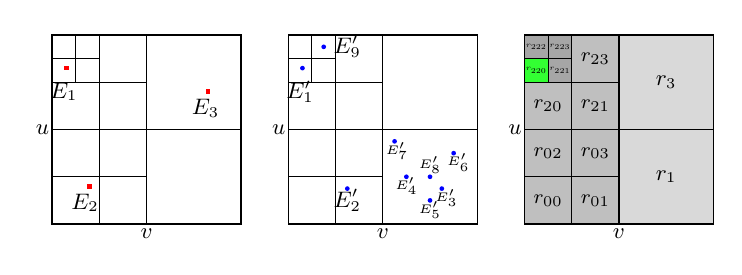
\begin{tikzpicture}[scale=0.3, every node/.style={scale=0.9}]
	% \draw[gray, very thin] (0,0) grid +(8,8);

	\begin{scope}[shift={(0,0)}]
	\draw (0,0) rectangle +(8,8);
	\draw[step=4] (0,0) grid +(8,8);
	\draw[step=2] (0,0) grid +(4,4);
	\draw[step=2] (0,4) grid +(4,4);
	\draw[step=1] (0,6) grid +(2,2);
    
	\fill[red!100] (0.5,6.5) rectangle +(0.2,0.2);
	\node at (0.5, 5.6) {\small $E_1$};
	\fill[red!100] (1.5,1.5) rectangle +(0.2,0.2);
	\node at (1.4, 0.9) {\small $E_2$};
	\fill[red!100] (6.5,5.5) rectangle +(0.2,0.2);
	\node at (6.5,4.9) {\small $E_3$};
	
	\node at (4,-0.4) {\small $v$};
	\node at (-0.4,4) {\small $u$};
	\end{scope}	 	
	
	\begin{scope}[shift={(10,0)}]
	\draw (0,0) rectangle +(8,8);
	\draw[step=4] (0,0) grid +(8,8);
	\draw[step=2] (0,0) grid +(4,4);
	\draw[step=2] (0,4) grid +(4,4);
	\draw[step=1] (0,6) grid +(2,2);
    
	\fill[blue!100] (0.6,6.6) circle (0.1);
	\node at (0.5, 5.6) {\small $E'_1$};
	\fill[blue!100] (2.5,1.5) circle (0.1);
	\node at (2.5, 1) {\small $E'_2$};
	\fill[blue!100] (6.5,1.5) circle (0.1);
	\node at (6.7, 1.1) {\tiny $E'_3$};
	\fill[blue!100] (5,2) circle (0.1);
	\node at (5, 1.6) {\tiny $E'_4$};
	\fill[blue!100] (6,1) circle (0.1);
	\node at (6, 0.6) {\tiny $E'_5$};
	\fill[blue!100] (7,3) circle (0.1);
	\node at (7.2, 2.6) {\tiny $E'_6$};
	\fill[blue!100] (4.5,3.5) circle (0.1);
	\node at (4.6, 3.1) {\tiny $E'_7$};
	\fill[blue!100] (6,2) circle (0.1);
	\node at (6, 2.5) {\tiny $E'_8$};
	\fill[blue!100] (1.5,7.5) circle (0.1);
	\node at (2.5, 7.5) {\small $E'_9$};
	
	\node at (4,-0.4) {\small $v$};
	\node at (-0.4,4) {\small $u$};
	\end{scope}

	\begin{scope}[shift={(20,0)}]
	\fill[gray!30] (0,0) rectangle +(8,8);
	\fill[gray!50] (0,0) rectangle +(4,4);
	\fill[gray!50] (0,4) rectangle +(4,4);
	\fill[gray!70] (1,6) rectangle +(1,1);
	\fill[gray!70] (1,7) rectangle +(1,1);
	\fill[gray!70] (0,7) rectangle +(1,1);
	\fill[green!80] (0,6) rectangle +(1,1);
	
	\draw (0,0) rectangle +(8,8);
	\draw[step=4] (0,0) grid +(8,8);
	\draw[step=2] (0,0) grid +(4,4);
	\draw[step=2] (0,4) grid +(4,4);
	\draw[step=1] (0,6) grid +(2,2);
	
	\node at (6,2) {\small $r_1$};
	\node at (6,6) {\small $r_3$};
	\node at (1,1) {\footnotesize $r_{00}$};
	\node at (3,1) {\footnotesize $r_{01}$};
	\node at (1,3) {\footnotesize $r_{02}$};
	\node at (3,3) {\footnotesize $r_{03}$};
	\node at (1,5) {\footnotesize $r_{20}$};
	\node at (3,5) {\footnotesize $r_{21}$};	
	\node at (3,7) {\footnotesize $r_{23}$};
	\node[scale=0.6] at (0.5,6.5) {\tiny $r_{220}$};
	\node[scale=0.6] at (1.5,6.5) {\tiny $r_{221}$};
	\node[scale=0.6] at (0.5,7.5) {\tiny $r_{222}$};
	\node[scale=0.6] at (1.5,7.5) {\tiny $r_{223}$};
	
	\node at (4,-0.4) {\small $v$};
	\node at (-0.4,4) {\small $u$};
	\end{scope}
	
	\end{tikzpicture}
\caption{\label{fig_radix_bucketing}From left to right: Elements of edge list $E$ with the bucket traversal overlay; elements of edge list $E'$ with the bucket traversal overlay; bucket traversal with region labels.}
\end{figure}

To perform bucketing, we first take the integer $u$ and mask the highest bit. The resultant value is concatenated with the masked highest bit of $v$. The resultant value is a number between 0 and 3. This lets us put each value in $E$ and $E'$ into the buckets $r_0$ through $r_3$ as shown in the last figure in figure \ref{fig_radix_bucketing}. From this point we will recursively compute intersections only if both $E$ and $E'$ have edges in the bucket. As shown in the first and second of figure \ref{fig_radix_bucketing} we can see that bucket $r_1$ in $E$ does not have any edges while bucket $r3$ in $E'$ does not have any edges. Hence, we do not need to recurse in these buckets at all. Now $r_1$ has edges $E'_3$ through $E'_8$ which do not need to be tested. We have eliminated the need to test 6 out of 9 edges in $E'$. This is a significant reduction in work. Also, $r_3$ is eliminated as a potential bucket for recursion in $E$ removing the need to test edge $E_3$. In the next level of recursion we eliminate buckets $r_{00}$ through $r_{03}$ as well as $r_{20}, r_{21}, r_{23}$. Recursing on $r_{22}$ further we see that $r_{220}$ is the only bucket which has edges both in lists $E$ and $E'$. $E'_9$ in bucket $r_{223}$ does not have corresponding edges in $E$. Since $r_{220}$ has very few elements in both $E$ and $E'$ we can compare each element in $E'$ to each element in $E$ for $r_{220}$ to find that $E'_1$ has a matching edge $E_1$ and is the only edge also present in list $E$.

Although this is a synthetic example, it demonstrates that sparse distributions on $E$ and $E'$ will result in elimination of a large set of candidates for intersection quickly. Each level of recursion is $O(|E|+|E'|)$ i.e. it is $O(n)$ in the size of the lists.

% \section{Background and Related work}
% \subsection{Parallel Graph algorithms}
% \subsection{GPU}
% \subsection{Linear algebra}
% \subsection{Graph}
% \subsection{Triangle counting}

\section{Methods}
\subsection{Simple Linear algebra approach as a motivation}
The problem of finding the count of triangles can be reduced to counting all paths(walks) of length 2 between two vertices if there is a closure i.e. an edge between the two vertices. An element $A(i,j)$ in the square adjacency matrix defines the number of paths or the weight of an edge between nodes $i$ and $j$. For an undirected unweighted graph the adjacency matrix elements are 0 or 1. We know that the $n^{th}$ power of an adjacency matrix $A^n$ gives us the number of walks $A^n(i,j)$ of length $n$ that exist between nodes $i$ and $j$. For $n=2$ the walks are paths if the diagonal of the adjacency matrix is 0. Thus, each element of $A^2$ defines the number of paths of length 2. Let $C$ denote the Hadamard product or elementwise product of this with the adjacency matrix $C=A^2\circ A$. An element of matrix $C(i,j)$ gives us he number of triangles edge $(i,j)$ is a part of. Hence, the sum of all the elements of this matrix gives us the total number of triangles in the graph. Each triangle is counted three times in the matrix $C$ - once for each edge. Also, in an undirected graph each edge is counted twice as $A(i,j)$ and $A(j,i)$ both indicating the same edge. This implies that $\sum_{ij}(C)$ counts each triangle $6$ times. The total number of triangles is given by equation \ref{numTriangles}:

\begin{equation}
 n_{T} = \sum_{ij}(C)/6 \label{numTriangles}
\end{equation}

Triangle counting using this method has a high work complexity and is viable only for graphs with dense adjacency matrices. Most graphs tend to have sparser adjacency matrices. We can reduce the work complexity by techniques such as using masked multiplication after LU decomposition\cite{b10}. The decomposition as well as the masked multiplication is computationally expensive since it uses a significant amount of communication between workers. We can reduce the amount of communication by using a set intersection approach.

\subsection{Short summary of standard algorithms}
Our algorithm consists of two main steps. The first step involves finding out all the possible combinations of wedges that exist in our graph. This is computed using the adjacency list representation of the graph. The result of this step is a list of edges closing the wedges hence forming a triangle. The second step is the radix bucket based set intersection. In this step we find out if the list of candidate edges computed before is actually present in the graph. The following sections describe these steps in detail.

\subsection{Finding candidate closure edges $E'$}
While generating the set of candidate edges we have focussed on maintaining exclusive access to the input and output buffers as well as coalescing our reads and writes. This ensures that the memory accessess which are sequential  will benifit from hierarchical memory caches in GPU architectures. Ensuring exclusive read and exclusive writes for large $E$ and $E'$ requires us two know two things. The size of the $E'$ output buffer to allocate in the global memory. The read boundaries of $E$ in which each thread will operate to generate the wedges along with the write boundaries of $E'$ where it will write the candidate edges closing these wedges. This is performed by the algorithm \ref{eprimegen}.

\begin{algorithm}
  \caption{Compute candidate edges for closure test.\label{eprimegen}}  
  \begin{algorithmic}[1]
    \Statex
    \Function{Compute\_$E'$}{$E$}
      \State $E$ $\gets$ RADIX\_SORT($E$) \Comment{\small $E(u, v)$ by $u$ first then $v$} \label{cubs_radix_sort}
      \State $cnt[p]$ $\gets$ PARALLEL\_COUNT($E$) \Comment{\small use transitions} \label{par_cnt}
      \State $E_{len}$ $\gets$ PARALLEL\_REDUCE($cnt[p]$) \label{par_red}
      \State ALLOCATE($E_{index}, E_{degree}, E'_{size}$) \Comment{\small size $E_{len}$}
      \State $E_{index}$ $\gets$ PARALLEL\_OFFSETS($E$, $p$) \label{par_offset}
      \State $E_{degree}$ $\gets$ PARALLEL\_DEGREE\_CALC($E_{index}$, $p$) \label{par_deg_calc}
      \State $E'_{size}$ $\gets$ PARALLEL\_SIZE\_CALC($E_{degree}$, $p$) \label{par_size_calc}
      \State $E'_{size\_scan}$ $\gets$ INCLUSIVE\_SUM\_SCAN($E'_{size}$)
      \State $E'$ $\gets$ PARALLEL\_GEN($E$, $E_{index}$, $E'_{size\_scan}$) \label{par_gen}
      \State \Return{$E'$}
    \EndFunction
  \end{algorithmic}
\end{algorithm}

The input to algorithm \ref{eprimegen} is the edge list $E$. Each element in the list $E$ is an ordered tuple $(u,v)$ representing a pair of vertices. If the number of vertices in the graph fit within the bounds of an integer container, a single element of $E$ can be interpreted as a long integer. Accounting for endianness might require reordering $(u,v)$ to $(v,u)$. The radix sort in line \ref{cubs_radix_sort} is performed on the edge list $E$ using the fast double buffered tunable radix sort from \cite{b19}. The resultant list is the adjacency list since it is sorted by $u$ first and $v$ next. We refer to the adjacency list as $E$ from here onwards. Since radix sort has a work complexity of $O(bn)$ where $b$ is the number of bits in the container which is fixed, the asymptotic work complexity of radix sort is $O(n)$. The parallel time complexity of this shared memory implementation is $O(n/p)$ where $p$ is the number of threads executing simultaneously. In steps \ref{par_cnt} and \ref{par_red}, the total number of vertices which is the length of the first dimension of the adjacency list $E_{len}$ is found. The next 4 steps are used to calculate the indexes in the input buffer $E_{index}$ and output buffer $E'_{size\_scan}$. 

Each step from \ref{par_offset} through \ref{par_size_calc} is performed in the same kernel although they have been explicitly separated. In line \ref{par_offset} the $p$ processors compute the index locations of the beginning of the adjacency list of each vertex and write the result to $E_{index}$. The difference between consecutive index values in $E_{index}$ is used in line \ref{par_deg_calc} to compute the degree of each vertex. The number of wedges centered on a vertex in the adjacency list is dependent on the degree of the vertex. For each vertex in the adjacency list, a wedge can be formed by selecting one other edge in the adjacency list. We can remove duplicate wedges by only considering the ${deg \choose 2}=\frac{deg(deg-1)}{2}$ combinations instead of the $deg^2$ permutations. The number of candidate edges is the number of closing edges which is 1 for each wedge. This value is computed in \ref{par_size_calc} and stored in $E'_{size}$.

The inclusive scan sum of $E'_{size}$ gives us the index locations in $E'$ where the combinations corresponding to each vertex in the adjacency list will be written. The inclusive sum is computed using \cite{b19}. In the final step in line \ref{par_gen}, each thread takes ownership of one or more vertices in the adjacency list $E$. For each vertex $u$ having degree $deg$ in the adjacency list, the $\frac{deg(deg-1)}{2}$ combinations of edges corresponding to wedges will be written out to the index locations in $E'$ pointed out by $E'_{size\_scan}$.

% Compute Eprime(Adjacency list E with each member being an ordered tuple of base type such as (u=int, v=int), ITEMS_PER_THREAD):
% 1. Read in the adjacency list as a list of double precision type.
% 2. Sort the adjacency list in place by u first and then v using cub:sortkey -> cite refs
% 3. Divide sorted E into equal sized chunks based on the amount of work to be done by each thread.
% 4. Find the length of the adjacency list. To do that basically find the number of unique u's in your chunk. In the next step we will add all the counts.

% 5. Reduce sum the counts to find the length of adjacency list. Allocate arrays of size |Adjacency list| for index, degree, EPrimeSize.

% 6. For the same chunks as in step 3 find the degree as well as the E array index. Also, in EPrimeSize array store the value d(d-1)/2 where d is degree at an index location.

% 7. Each vertex in the adjacency list will produce deg(deg-1)/2 combinations that are stored in EPrimeSize. We have to generate the index locations at which we will write the outputs which will be EPrimeSizeScan.
% 8. EPrimeSizeScan = Inclusive sum scan(EPrimeSize)

% 9. We perform a division based on the amount of work which uses e_index but do not mention it in this iteration.
% 10. Read from sorted E and each thread will generate the combinations in the adjacency list of the particular u and write it out to a buffer using EPrimeSizeScan.
% 11. Return the list of all possible combinations called EPrime.


\subsection{Set intersection using radix bucketing}
Counting of the triangles is done by finding out if each edge in $E'$ is actually present in $E$. Performing a lookup for each member from $E'$ in $E$ can be a $O(|E'|log(|E|))$ operation if $E$ is sorted using a naive binary tree. But $E$ itself can be very large and may not fit in memory even if we batch the lookups of members of $E'$. In this case we need an algorithm which can scale well and work on shared as well as distributed memory architectures. Although our implementation is on a shared memory SIMD device, we have designed the algorithm to be extended onto distributed memory SPMD architectures. The motivation for our algorithm is the MSD bucketing algorithm which is at the core of the fastest sorting algorithms\cite{b14}. It is easy to split up the work among threads with a low communication overhead between recursion and threads. Note that this algorithm is recursive. It fits very well with the NVIDIA CUDA Dynamic Parallelism extension\cite{b21}. The algorithm is shown in \ref{tri_count}.

\begin{algorithm}
  \caption{Count triangles by counting $|E \cap E'|$.\label{tri_count}}
  \begin{algorithmic}[1]
    \Statex
    \State $t\_cnt = 0$ 
    \State $b=2^d$ \Comment{\small $d=$ radix bits, $b=$ radix buckets}
    \Function{INTERSECT\_COUNT}{$E, E', t\_cnt, depth$}
      \If{$|E|=0 \land |E'|=0$} \label{recursion_term_empty}
	\State \Return{}
      \EndIf
      \If{$depth \geq depth_{max}$ \label{recursion_term_dmax}}
	\State $t\_cnt = t\_cnt + |E'|$
	\State \Return{}
      \EndIf
      \If{$|E|\leq thr \lor |E'|\leq thr$ \label{recursion_term_thresh}}
	\State $t\_cnt = t\_cnt +$SEQ\_INTERSECT\_CNT($E, E'$)
	\State \Return{}
      \EndIf
      \State $E_{cnt}[b]$ $\gets$ PARALLEL\_COUNT($E$, $depth$) \label{par_cnt_e}
      \State $E'_{cnt}[b]$ $\gets$ PARALLEL\_COUNT($E'$, $depth$) \label{par_cnt_e_prime}
      \State $E_{cnt\_scan} \gets$ $vec^{-1}($INC\_SUM\_SCAN$(vec(E^T_{cnt})))$ \label{inc_sum_scan_e_cnt}
      \State $E'_{cnt\_scan} \gets$ $vec^{-1}$(INC\_SUM\_SCAN$(vec(E'^T_{cnt}))$) \label{inc_sum_scan_e_prime_cnt}
      \ForAll{b}
	\State $E_{buf}[b] \gets$ MOVE($E, E_{cnt\_scan}[b]$) \label{move_e_cnt_scan}
      \EndFor
      \ForAll{b}
	\State $E'_{buf}[b] \gets$ MOVE($E', E'_{cnt\_scan}[b]$) \label{move_e_prime_cnt_scan}
      \EndFor
      \ForAll{b}
	\State INTERSECT\_COUNT($E_{buf}[b], E'_{buf}[b], t\_cnt, depth+1$) \label{recursion_call}
      \EndFor
    \EndFunction
  \end{algorithmic}
\end{algorithm}

The triangle count $t\_cnt$ is initialized to 0 and it will be updated atomically by the threads as they find valid candidate edges in $E'$. We can specify the number of radix bits and hence the number of buckets to use for the algorithm up front. The recursive function takes as parameters the edge list $E$, the candidate edge list $E'$, the pointer to the triangle count $t\_cnt$ and the current depth of the recursion $depth$. Early recursion termination happens on lines \ref{recursion_term_empty}, \ref{recursion_term_dmax} and \ref{recursion_term_thresh}. The termination conditions on lines \ref{recursion_term_empty}, \ref{recursion_term_dmax} are self-explanatory. A hybrid approach towards the tail end of the recursion is known to perform better\cite{b16}. When the input is small i.e. $|E|$ and $|E'|$ are smaller than a threshold $thr$ we perform a simple sequential intersection count and add it to $t\_cnt$. Although we have not implemented it, its worth mentioning that the OrderedMerge demonstrated in \cite{b17, b18} are alternatives that can yield substantial improvements at the tail end of the recursion.

The first step of the recursion is the parallel count. The parallel count in lines \ref{par_cnt_e} and \ref{par_cnt_e_prime} distributes the input list among $p$ threads. Each thread will process $\frac{n}{p}$ edges. A simple masking operation for the vertices of each edge as shown in \ref{bucket_mask} tells us the bucket to which $q$ will belong

\begin{equation}
(q \gg (2^{depth_{max}-depth}-(d-1)))\land(b-1) \label{bucket_mask}
\end{equation}

The $b$ counts $E_{cnt}$, $E'_{cnt}$  shown in line \ref{par_cnt_e} will be populated with a time complexity $O(\frac{|E|}{p})$ and $O(\frac{|E'|}{p})$ assuming the $p$ threads work simultaneously. This count is computed in global shared memory and is a matrix of size $p \times b$ since the local count computed by each thread is not summed up yet. For the move to be performed in parallel by $p$ threads in lines \ref{move_e_cnt_scan} and \ref{move_e_prime_cnt_scan}, we need to know the index location in the output buffers $E_{buf}$ and $E'_{buf}$ where the data will be moved.

The steps in lines \ref{inc_sum_scan_e_cnt}, \ref{inc_sum_scan_e_prime_cnt} perform the task of computing the index locations of the move. The operator $vec$ used in line \ref{inc_sum_scan_e_cnt} is the vectorization operator\cite{b20} that will convert the $p \times b$ matrix into a column vector of size $bp \times 1$. An inclusive scan of this vector gives us the index location boundaries where each thread will perform a move operation for each bucket. The inclusive sum scan has a work complexity of $O(pb\cdot log(pb))$ and a time complexity defined by the Kogge-Stone or Hillis-Steele scan algorithms \cite{b14}. This enables us to perform the move as an EREW(exclusive read, exclusive write) operation in the final step. The $vec^{-1}$ operator simply converts the $bp \times 1$ vector into a $p \times b$ matrix. Note that the $vec$ and $vec^{-1}$ and transpose operations do not have to be performed explicitly if the $E_{cnt}$ is stored in column major order.

The last step before recursion is the data movement. In line \ref{move_e_cnt_scan} the edges in $E$ are moved based on the bucket they belong to the offsets pointed by $E_{cnt\_scan}$ in the output buffer $E_{buf}$. The move is done for $E'$ in line \ref{move_e_prime_cnt_scan}. This stable operation requires just two buffers of size $2\times (|E|+|E'|)$ since the input buffer at $depth$ can be used as the output buffer at recursion $depth+1$ and vice versa.

Intersect\_count will be called recursively for each bucket with the corresponding data as shown in line \ref{recursion_call}. The pointer to a global memory $t\_cnt$ is also passed on. The recursive call is made to all the buckets simultaneously - the loop over all buckets has only been shown for clarity. Similarly, the loops in lines \ref{move_e_cnt_scan}, \ref{move_e_prime_cnt_scan} also run simultaneously.

% Radix sort count E and EPrime(E, EPrime, len_E, len_EPrime, triangleCount, depth):
% 1. If len_E or len_EPrime is 0 return.
% 2. If the this recursion goes beyond the depth_max simple add the count len_EPrime to triangleCount and return.
% 3. If the number of elements in len_E or len_EPrime is smaller than a threshold perform a lookup for each element in EPrime in E in O(len_E*len_EPrime). Add count to trianglecount and return.
% 4. Find counts for each bucket in the list E and list EPrime using radix bucketing.

% 5. Prefix inclusive sum scan for both E and EPrime.
% 6. Move the elements in E and EPrime to their respective buckets.
% 7. Recurse for each bucket.

\section{Results and conclusion}
\subsection{Effect of changing the size of sets $|E|$ and $|E'|$ on the running time}
To test scaling we demonstrate the effect of changing two major properties of the graph. The number of edges $|E|$ in the graph and the density of the graph which changes as $|E'|$ changes. In the first set of values shown in table \ref{table_result_runtimes} we can see that the increasing the number of edges as well as the density i.e. correspondingly the size of $E'$ does not have a significant impact on the time taken to COMPUTE\_$E'$. The INTERSECTION\_COUNT also takes roughly the same amount of time although it is a bit more unpredictable. The change in the time takes by INTERSECTION\_COUNT can be attributed to the maximum recursion depth at which the recursion terminates. In set 2 the outliers from set 1 have been showcased. This rapid increase in the runtime is caused due to incorrect tuning of kernels. We are currently working on tuning the kernels to give a uniform performance irrespective of input size and density. It should be noted that the number of triangles in the actual graph does not really have an effect on the running time. The running time for dataset Theory-25-81-Bk.tsv at 59.5 s is close to the running time of Theory-25-81-B1k.tsv at 66.16 s. The difference in the number of triangles 0 against 2025 does not reduce the running time.
\begin{table*}[ht]
\centering
 \begin{tabular}{|c || c | c | c || c | c | c |} 
 \hline
 \multicolumn{4}{|c||}{}&\multicolumn{3}{|c|}{Run time in seconds} \\
 \hline
 Dataset & $\#edges |E|$ & size of $|E'|$ & $\#triangles$ & COMPUTE\_$E'$ & INTERSECT\_COUNT & Total \\ [0.5ex] 
 \hline\hline
 Theory-3-4-Bk.tsv & 48 & 96 & 0 & 0.6 & 0.4 & 0.66 \\
 \hline
 Theory-3-4-5-Bk.tsv & 480 & 3360 & 0 & 0.61 & 0.08 & 0.71 \\
 \hline
 Theory-16-25-Bk.tsv & 1600 & 87600 & 0 & 0.63 & 0.11 & 0.76 \\
 \hline
 Theory-3-4-5-9-Bk.tsv & 8640 & 319680 & 0 & 0.63 & 0.36 & 1.04 \\
 \hline
 Theory-3-4-B1k.tsv & 62 & 225 & 36 & 0.6 & 0.03 & 0.67 \\
 \hline
 Theory-3-4-5-B1k.tsv & 692 & 10830 & 287 & 0.6 & 0.09 & 0.71 \\
 \hline
 Theory-16-25-B1k.tsv & 1682 & 105620 & 400 & 0.62 & 0.2 & 0.84 \\
 \hline
 Theory-3-4-B2k.tsv & 62 & 138 & 1 & 0.61 & 0.4 & 0.67 \\
 \hline
 Theory-3-4-5-B2k.tsv & 692 & 5339 & 7 & 0.61 & 0.08 & 0.71 \\
 \hline
 Theory-16-25-B2k.tsv & 1682 & 88943 & 1 & 0.62 & 0.13 & 0.78 \\
 \hline
 Theory-3-4-5-9-B2k.tsv & 13166 & 522804 & 35 & 0.64 & 0.79 & 1.48 \\
 \hline\hline
 
 Theory-3-4-5-9-B1k.tsv & 13166 & 1223427 & 9107 & 0.73 & 11.99 & 12.76 \\
 \hline
 Theory-25-81-Bk.tsv & 8100 & 2154600 & 0 & 0.87 & 58.59 & 59.5 \\
 \hline
 Theory-25-81-B1k.tsv & 8312 & 2378865 & 2025 & 0.9 & 65.220001 & 66.160004 \\
 \hline
 Theory-25-81-B2k.tsv & 8312 & 2165433 & 1 & 0.9 & 58.91 & 59.860001 \\
 \hline\hline\hline

 p2p-Gnutella04\_adj.tsv & 79988 & 518694 & 934 & 0.55 & 2.02 & 2.75 \\
 \hline
 p2p-Gnutella05\_adj.tsv & 63678 & 439066 & 1112 & 0.59 & 1.88 & 2.62 \\
 \hline
 p2p-Gnutella06\_adj.tsv & 63050 & 422567 & 1142 & 0.55 & 1.56 & 2.26 \\
 \hline
 p2p-Gnutella08\_adj.tsv & 41554 & 346033 & 2383 & 0.56 & 1.8 & 2.47 \\
 \hline
 p2p-Gnutella09\_adj.tsv & 52026 & 411347 & 2354 & 0.55 & 1.7 & 2.38 \\
 \hline
 p2p-Gnutella25\_adj.tsv & 109410 & 533121 & 806 & 0.55 & 1.98 & 2.76 \\
 \hline\hline

 p2p-Gnutella30\_adj.tsv & 176656 & 923756 & 1590 & 0.54 & 3.47 & 4.33 \\
 \hline
 p2p-Gnutella31\_adj.tsv & 295784 & 1568174 & 2024 & 0.54 & 5.66 & 6.95 \\
 \hline
\end{tabular}
 \caption{Four sets of results. The first set consists of graphs with zero, many and some triangles in that order. The second consists of the outliers from the first set. The third collection represents graphs where the number of edges varies as well as the size of the set $E'$ varies but the running time is roughly constant. The last set contains outliers; the number of edges as well as the size of $E'$ generated doubles causing run time to double and triple.}
 \label{table_result_runtimes}
\end{table*}

\subsection{Effect of changing the structure of the graph on the running time}
The p2p-Gnutella dataset has roughly the same density and connectivity since $|E'|$ is about 450000 while the number of edges range from 40000 to about 100000. This can be seen in the third set of the results. As seen in the total running time the structure and connectivity characteristics do not have a significant effect on the running time which is constant at about 2.5 seconds as seen in table \ref{table_result_runtimes}. The set 4 shows some of the outliers. But we can see that the COMPUTE\_$E'$ function still takes the same time. The minor differences in the INTERSECT\_COUNT can be attributed to the recursion depth and early termination. 

\subsection{Conclusion}
The strategy to generate the offsets where we can read from and write processed results can be effectively applied for various parallel tasks. It is scalable as can be seen by the run timings for similar graphs in table \ref{table_result_runtimes}. The recursive radix sort is not performing adequately due to a bug in tuning the kernel. 
We intend on fixing the issue by batching the stage of generation of $|E'|$ and performing the intersection count.

\begin{thebibliography}{00}
\bibitem{b1} D. Watts and S. Strogatz, “Collective dynamics of ’small-world’ networks,” Nature, no. 393, 1998.
\bibitem{b2} Adam Polak, “Counting Triangles in Large Graphs on GPU.“
\bibitem{b3} Ron Milo, Shai Shen-Orr, Shalev Itzkovitz, Nadav Kashtan, Dmitri Chklovskii, Uri Alon, Network motifs: Simple building blocks of complex networks, Science 298 (2002) 824–827
\bibitem{b4} ] Thomas Schank, Dorothea Wagner, Finding, counting and listing all triangles in large graphs, Technical report, Universität Karlsruhe, Fakultät für Informatik, 2005.
\bibitem{b5} M. Bisson and M. Fatica, "Static graph challenge on GPU," 2017 IEEE High Performance Extreme Computing Conference (HPEC), Waltham, MA, 2017, pp. 1-8.
\bibitem{b6} “Static Graph Challenge: Subgraph Isomorphism”, S. Samsi, V. Gadepally, M. Hurley, M. Jones, E. Kao, S. Mohindra, P. Monticciolo, A. Reuther, S. Smith, W. Song, D. Staheli, J. Kepner, IEEE High Performance Extreme Computing Conference (HPEC), 2017
\bibitem{b7}  O. Green, P. Yalamanchili, and L.-M. Munguıa, “Fast triangle counting on the GPU,” in Proc. 4th Workshop Irregular Appl.: Archit. Algorithms, 2014, pp. 1–8. [Online]. Available: http://dx.doi.org/ 10.1109/IA3.2014.7
\bibitem{b8} Static Graph Challenge on GPU, Mauro Bisson, Massimiliano Fatica
\bibitem{b9} L. Wang, Y. Wang, C. Yang, and J. D. Owens, “A comparative study on exact triangle counting algorithms on the GPU,” in Proc. 1st High Performance Graph Process. Workshop, May 2016, pp. 1–8.
\bibitem{b10} Azad, A. Buluc¸, and J. Gilbert, “Parallel triangle counting and enumeration using matrix algebra,” in Proc. IEEE Int. Parallel Distrib. Process. Symp. Workshop, 2015, pp. 804–811. [Online]. Available: http://dx.doi.org/10.1109/IPDPSW.2015.75
\bibitem{b11} T. G. Kolda, A. Pinar, T. Plantenga, C. Seshadhri, and C. Task, “Counting triangles in massive graphs with mapReduce,” CoRR, 2013. [Online]. Available: http://arxiv.org/abs/1301.5887
\bibitem{b12}  C. Seshadhri, A. Pinar, and T. G. Kolda, “Wedge sampling for computing clustering coefficients and triangle counts on large graphs,” Statistical Anal. Data Mining, vol. 7, no. 4, pp. 294–307, 2014. [Online]. Available: http://dx.doi.org/10.1002/sam.11224
\bibitem{b13} M. Jha, C. Seshadhri, and A. Pinar, “A space-efficient streaming algorithm for estimating transitivity and triangle counts using the birthday paradox,” ACM Trans. Knowl. Discov. Data, vol. 9, no. 3, pp. 15:1–15:21, Feb. 2015. [Online]. Available: http://doi.acm. org/10.1145/2700395
\bibitem{b14} V. J. Duvanenko, "Parallel In-Place Radix Sort Simplified", Dr. Dobb's Journal, January 2011
\bibitem{b15} Single-pass Parallel Prefix Scan with Decoupled Look-back, Duane Merrill, Michael Garland
\bibitem{b16} V. J. Duvanenko, "Stable Hybrid N-bit-Radix Sort", Dr. Dobb's Journal, January 2010
\bibitem{b17} J. Shun and K. Tangwongsan, “Multicore triangle computations without tuning,” in Data Engineering (ICDE), 2015 IEEE 31st International Conference on. IEEE, 2015, pp. 149–160.
\bibitem{b18} A. S. Tom et al., "Exploring optimizations on shared-memory platforms for parallel triangle counting algorithms," 2017 IEEE High Performance Extreme Computing Conference (HPEC), Waltham, MA, 2017, pp. 1-7.
\bibitem{b19} \url{https://nvlabs.github.io/cub/structcub_1_1_device_radix_sort.html}
\bibitem{b20} H.D. Macedo, J.N. Oliveira, Typing linear algebra: A biproduct-oriented approach, Science of Computer Programming, Volume 78, Issue 11, 2013, Pages 2160-2191.
\bibitem{b21} \url{https://docs.nvidia.com/cuda/cuda-c-programming-guide/index.html#cuda-dynamic-parallelism}
\end{thebibliography}
\end{document}
